\documentclass{article}
\usepackage[utf8]{inputenc}
\usepackage[spanish]{babel}
\usepackage{listings}
\usepackage{graphicx}
\graphicspath{ {images/} }
\usepackage{cite}

\begin{document}

\begin{titlepage}
    \begin{center}
        \vspace*{1cm}
            
        \Huge
        \textbf{}
            
        \vspace{0.5cm}
        \LARGE
        Subtítulo
            
        \vspace{1.5cm}
            
        \textbf{Mateo Cardona Correa}
            
        \vfill
            
        \vspace{0.8cm}
            
        \Large
        Despartamento de Ingeniería Electrónica y Telecomunicaciones\\
        Universidad de Antioquia\\
        Medellín\\
        Abril de 2021
            
    \end{center}
\end{titlepage}

\tableofcontents
\newpage
\section{Introduccion al Trabajo}\label{intro}
El trabajo aqui presentado se realiza bajo la consideracion de la presentacion de un problema planteado en la normativa de la cotidianidad, presentando un problema tan comun como puede ser el desarrollo de un cartel publicitario luminoso LED o el simple problema de manejo de una pantalla de caracteristicas basicas.

\subsection{Analisis del problema}\label{}
El problema aqui planteado tiene una serie de problemas a desarrollar, tales como\\
    -El manejo de multiples componentes electronicos basicos, tales como Leds y resistencias\\
    -El manejo de componentes electronicos mas avanzados, tales como un circuito integrado y una placa Arduino\\
    -La forma de implementar componentes electronicos y la utilizacion de programacion tipo C++
\subsection{Variantes a considerar}\label{}
Las variantes mas importantes a considerar fueron\\
    -El verificar el funcionamiento mas basico de los componentes electronicos conectados\\
    -La forma y el funcionamiento del codigo fuente\\
    -Funcionamiento en conjunto tanto del hardware como del software\\
    -Pequeños errores e imprevistos que pudieron haber surgido a lo largo del proyecto
\newpage
\section{Sección de contenido} \label{contenido}
Esta sección es para agregar toda la información correspondiente con código, citas, etc.
\subsection{Esquema}
El esquema realizado fue el siguiente:\\
Menu Inicial:\\
    -Demostracion\\
    -Comando para verificar funcionamiento de los leds\\
    -Comando para apagar los leds\\
    -Ingreso manual de imagenes (De decimal a Binario)\\
    -Desarrollo de una animacion, con una lista de imagenes dadas

\subsection{Algoritmo/Codigo}
%
A continuación, se presenta el código creado para el desarrollo de la actividad \ref{codigo_ejemplo},
\begin{lstlisting}[language=C++, label=codigo_ejemplo]
// Programa desarrollado, compilado y ejecutado en 
https://www.tinkercad.com
/************************************
* Matriz de leds 8x8 con 2 74HC595
* Parcial 1 de Informatica 2
* Mateo Cardona
*************************************/

// pines del 74HC595
const int ClockPin_1 = 5; //SHCP
const int LatchPin_1 = 4; //STCP
const int DataPin_1 = 3;  //DS

const int ClockPin_2 = 12; //SHCP
const int LatchPin_2 = 11; //STCP
const int DataPin_2 = 10;  //DS

String a = "";
int set = 0, t = 0;
uint8_t aux[8];

// Algunas figuras para mostrar en la matriz en formato hexadecimal
uint8_t demo1[8] = { // H
  0xe7,
  0xe7,
  0xe7,
  0xff,
  0xff,
  0xff,
  0xe7,
  0xe7,
};

uint8_t demo2[8] = { // E
  0xff,
  0xff,
  0xe0,
  0xff,
  0xff,
  0xe0,
  0xff,
  0xff,
};

uint8_t demo3[8] = { // Y
  0xc3,
  0xe7,
  0x7e,
  0x3c,
  0x3c,
  0x3c,
  0x3c,
  0x3c,
};

uint8_t clearval[8] = { // Matriz apagada
  0x00,
  0x00,
  0x00,
  0x00,
  0x00,
  0x00,
  0x00,
  0x00,
};

uint8_t verif[8] = {
  0xff,
  0xff,
  0xff,
  0xff,
  0xff,
  0xff,
  0xff,
  0xff,
};

// SETUP con inicializacion de pines y serial en 9600
void setup()
{
  pinMode(ClockPin_1, OUTPUT);
  pinMode(LatchPin_1, OUTPUT);
  pinMode(DataPin_1, OUTPUT);
  
  pinMode(ClockPin_2, OUTPUT);
  pinMode(LatchPin_2, OUTPUT);
  pinMode(DataPin_2, OUTPUT);
  
  Serial.begin(9600);
  Serial.println("Bienvenido!");
  Serial.println("Para mostrar el mensaje de ayuda escriba 'h'");
}

// funcion para mostrar data[] en la matriz
void display(uint8_t data[])
{
  for(int j=0; j<8; j++){
    digitalWrite(LatchPin_2, LOW);
    digitalWrite(LatchPin_1, LOW);
    shiftOut(DataPin_2, ClockPin_2, LSBFIRST, ~0x80 >> j);
    shiftOut(DataPin_1, ClockPin_1, LSBFIRST, data[j]);
    digitalWrite(LatchPin_2, HIGH);
    digitalWrite(LatchPin_1, HIGH);
    delay(2);
  }
}

void demo()
{
  int t = 0;
  while(t < 2000){
    display(demo1);
    t += 32;
  }while(t < 4000){
    display(demo2);
    t += 32;
  }while(t < 6000){
    display(demo3);
    t += 32;
  }
}

void imagen(uint8_t* i)
{
  while(Serial.available() <= 0){
    i[0] = 0;
  }
  a = Serial.readString();
  Serial.println(a);
  String aaaa = "", nn = " ";
  int c = 0, x = 0;
  while(a[c]){
    if(a[c] == nn[0]){
      i[x] = aaaa.toInt();
      x++;
      aaaa = "";
    }else{
      aaaa = aaaa + a[c];
    }
    c++;
    if(x == 8)
      return;
  }
  i[x] = aaaa.toInt();
  aaaa = "";
}

void publik()
{
  int i = 0, t = 0, taux = 0;
  Serial.println("Ingrese la cantidad de patrones que quiere en la animacion");
  while(Serial.available() <= 0){
    i = 0;
  }
  a = Serial.readString();
  i = a.toInt();
  Serial.println("Ingrese el tiempo en milisegundos de cada cuanto cambia la imagen (1s = 1000ms)");
  while(Serial.available() <= 0){
    t = 0;
  }
  a = Serial.readString();
  t = a.toInt();
  uint8_t** auxs = new uint8_t*[i];
  for(int j = 0; j < i; j++)
    auxs[j] = new uint8_t[8];
  for(int j = 0; j < i; j++){
    Serial.println("Ingrese la imagen");
    imagen(aux);
    for(int k = 0; k < 8; k++){
      auxs[j][k] = (int) aux[k];
    }
  }
  Serial.println("Iniciando animacion");
  for(int j = 0; j < i; j++){
    while(taux < t*(j+1)){
      display(auxs[j]);
      taux += 32;
    }
  }
  Serial.println("animacion terminada");
  display(clearval);
  for(int j = 0; j < i; j++)
    delete[] auxs[j];
  delete[] auxs;
}

void loop()
{
  while(Serial.available() > 0){
    a = Serial.readString();
    Serial.println(a);

    if(a == "h" || a == "H"){
      Serial.println("Ingrese:");
      Serial.println("'h' para mostrar este mensaje de ayuda");
      Serial.println("'c' para apagar todos los leds");
      Serial.println("'demo' para ver una animacion de ejemplo con duracion de 6 segundos");
      Serial.println("'verificar' para verificar que todos los leds funcionan");
      Serial.println("'imagen' para ingresar una imagen personalizada y mostrarla en la matriz");
      Serial.println("'publik' para crear una animacion con n imagenes");
    }else if(a == "c" || a == "C"){
      Serial.println("Apagando todos los leds");
      set = 0;
    }else if(a == "verificar"){
      Serial.println("Encendiendo todos los leds para verificar el funcionamiento");
      set = 3;
    }else if(a == "demo"){
      Serial.println("Iniciando demostracion de la animacion de la palabra 'HEY'");
      demo();
      set = 0;
    }else if(a == "imagen"){
      Serial.println("Ingrese en formato decimal (0, 255), puede ayudarse de un conversor de binario a decimal.");
      display(clearval);
      imagen(aux);
      set = 1;
    }else if(a == "publik"){
      publik();
    }else{
      Serial.println("No es un comando valido");
    }
  }

  if(set == 3)
    display(verif);
  else if(set == 1)
    display(aux);
  else
    display(clearval);
}
\end{lstlisting}
\subsection{Problemas Presentados a lo largo del ejercicio}
Los problemas presentados a lo largo del ejercicio fueron varios, entre ellos estan:\\
-La forma de introducir las imagenes\\
-Verificar que la parte de "imagen" funcionara correctamente, desde la transformacion de decimal a binario, como la utilizacion de strings y de la memoria dinamica, para su correcta ejecucion\\
-La utilizacion tanto de los tiempos como de la combinacion Decimal-Binario para definir la utilizacion correcta de los LEDS
\subsection{Evolucion del Algoritmo}
El algoritmo implementado sufrio multiples modificaciones desde el inicio, variando principalmente en las formas en las que se iban presentando las dificultades, siendo la principal de ellas la eleccion de utilizar un sistema decimal 0-255 para definir la forma en como se entrarian las imagenes correspondientes, y se eligio mas por su simplicidad que por su sencilleza, siendo el otro gran problema presentado durante el desarrollo la implementacion correcta de la secuencia de imagenes en el parametro publik utilizado, esto debido al conocimiento y manejo de conceptos tales como memoria dinamica y punteros.
 El resto del algoritmo se realiza de una manera mas sencilla, tanto como el desarrollo del parametro "demo" como la verificacion del correcto funcionamiento de los leds, dejando por ultimo la creacion de un menu tipo terminal facil de utilizar
\ref{imagenes}
\section{Inclusión de imágenes} \label{imagenes}
En la Figura (\ref{fig:parcial1}), se presenta el desarrollo completo del circuito utilizado
\begin{figure}[h]
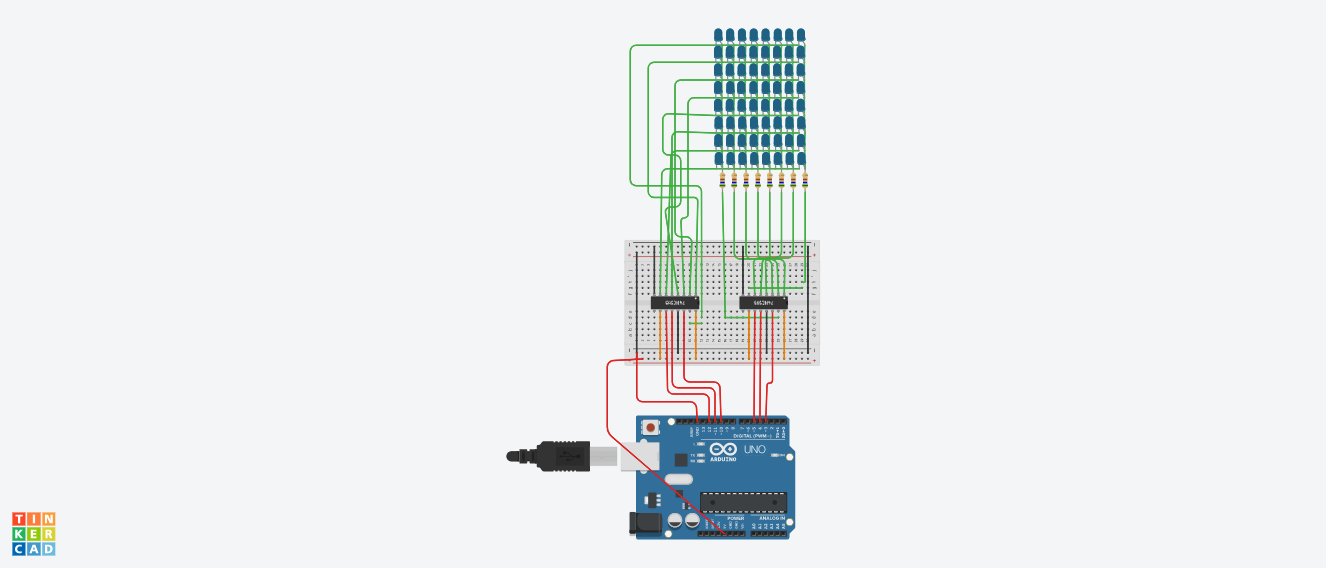
\includegraphics[width=4cm]{parcial1.png}
\centering
\caption{Logo de C++}
\label{fig:parcial1}
\end{figure}

Las secciones (\ref{intro}), (\ref{contenido}) y (\ref{imagenes}) dependen del estilo del documento.

\bibliographystyle{IEEEtran}
\bibliography{references}

\end{document}
